\chapter{Ιστορική Αναδρομή}


Τα γραφικά με υπολογιστές αποτελούσαν πάντα ένα πολύ χρήσιμο εργαλείο
για την παρουσίαση των αποτελεσμάτων των επιστημονικών υπολογισμών. Με τη σημερινή ανάπτυξη των υπολογιστών, τα γραφικά παίζουν πολύ σημαντικό ρόλο όχι πλέον μόνο σε επιστημονικές εφαρμογές αλλά και σε εμπορικές, όπως για παράδειγμα στα παιχνίδια και στο σχεδιασμό σελίδων στο διαδίκτυο.

Η έννοια γραφικά με υπολογιστές (computer graphics), δηλαδή να χρησιμοποιήσουμε έναν υπολογιστή για να δημιουργήσουμε μία εικόνα, ξεκίνησε από τις πρώτες μέρες των υπολογιστών. Ο επόμενος πίνακας μας δείχνει την εξέλιξη στο υλικό (hardware) των υπολογιστών που απαιτείται για την ανάπτυξη γραφικών. 

%Αρχική Χρήση: MIT Whirlwind 1951
%Graph Plotters:
%1953
%Έγχρωμες Οθόνες: 1962
%Τέλος 1960:
%1970:
%1980:
%Graphics hardware ακριβό
%τα γραφικά πολυτέλεια
%Time Sharing Συστήματα. Εισάγονται φθηνότερες μονάδες γραφικών. Tektronix 1968 Storage tube (terminal γραφικών 1024 x 768) Raster display (βασισμένο στην Τεχνολογία της Τηλεόρασης). Εύκολο editing στην εικόνα. Πιο φθηνά. Εισάγεται ως επιπλέον διάσταση το χρώμα. Για πρώτη φορά εκτυπώνονται χάρτες με σκίαση και όχι μόνο γραμμές. Εμφανίζονται: flat-bed plotters, ink-jet plotters, laser printers. Εμφάνιση μικροϋπολογιστών (simple user) και workstations (Apple Macintosh έως SUN workstation). Κυρίως σχεδιασμένα με δυνατότητες γραφικών σα θεμελιώδους μέρους στην κατασκευή. Στενός συνδυασμός επεξεργαστή - οθόνης γραφικών. Περιβάλλον για interactive εφαρμογές. Έχουμε και “graphical supercomputers”. Αυτά χρησιμοποιούν αρχιτεκτονική παράλληλης επεξεργασίας για να εξασφαλίσουν στο χρήστη δύναμη.

%
\begin{center}
	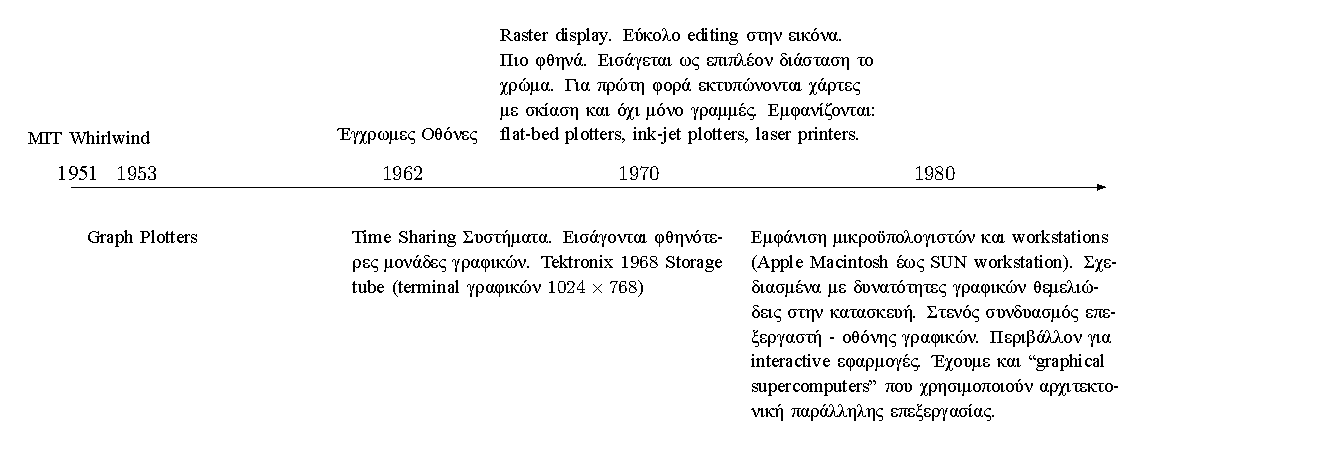
\includegraphics[scale=0.8]{/History/timelapse.pdf}
\end{center}

\subsection*{Λογισμικό (Software) Γραφικών}

Έχει αναπτυχθεί πάρα πολύ τα τελευταία 30 χρόνια. Αρχικά οι δυνατότητες ήταν πολύ περιορισμένες. Οι περισσότεροι κατασκευαστές hardware έδιναν τη δυνατότητα στην ύπαρξη μιας μικρής βιβλιοθήκης γραφικών (περιείχε συνήθως υπορουτίνες FORTRAN). Πολλοί κατασκευαστές εφοδίαζαν τον υπολογιστή με κάποιο πακέτο γραφικών το οποίο ήταν εξηρτημένο από την εκάστοτε μηχανή και δεν εκτελείτο σε διαφορετικό υπολογιστή (device-dependent). 

Προς το τέλος του 1960, αρχίζει να αναπτύσσεται λογισμικό γραφικών ανεξάρτητο από την εκάστοτε μηχανή (device-independent graphics software) και βιβλιοθήκες γραφικών (π.χ. GINO στην Μεγάλη Βρετανία). Το 1970 αποτελεί τη βάση για την ανάπτυξη βιβλιοθηκών γραφικών που δεν εξαρτώνται από την εκάστοτε μηχανή.

Σήμερα έχουμε ολοκληρωμένα πακέτα γραφικών π.χ. MATHCAD, CorelDRAW. Επίσης μέσα από μαθηματικά πακέτα υπολογισμού π.χ. MATLAB, MAPLE, MATHEMATICA μπορούν να δημιουργηθούν γραφικά.

\subsection{Η έννοια του pixel}

Ας εστιάσουμε τώρα στη βασική αρχή σχεδιασμού που χρησιμοποιείται στους υπολογιστές. Για την δημιουργία οποιασδήποτε εικόνας γραφικών είναι απαραίτητη η έννοια του pixel.

Ξεκινώντας από την αρχή ότι δεν μπορούμε να παραστήσουμε ένα άπειρο αριθμό σημείων σ' έναν υπολογιστή, περιοριζόμαστε πάντοτε σ' έναν πεπερασμένο αριθμό σημείων που θα απαρτίζει μία γραμμή (συνήθως όχι περισσότερα από μερικές εκατοντάδες ή χιλιάδες).

Ο μέγιστος αριθμός των διακεκριμένων σημείων που μπορεί να έχει μία γραμμή καθορίζει την ανάλυση (resolution) μιας μονάδας εξόδου (οθόνης). Όσο περισσότερα τα σημεία, τόσο υψηλότερη η ανάλυση της οθόνης. Αυτός ο περιορισμός δεν είναι τόσο καταστρεπτικός αφού το ανθρώπινο μάτι δε μπορεί να διακρίνει περισσότερα από 1000 σημεία σε κάθε ευθύγραμμο τμήμα.

Επομένως αφού πρέπει να κατασκευάζουμε τις γραμμές από πεπερασμένο αριθμό σημείων κάθε σημείο έχει κάποιες διαστάσεις και έτσι δεν είναι απλώς και μόνο σημείο. Το pixel, η ονομασία του οποίου προκύπτει από το ``Picture Element", είναι το μικρότερο στοιχείο της οθόνης που καθορίζεται από κάποια διεύθυνση και το οποίο μπορούμε να ελέγχουμε. Κάθε pixel χαρακτηρίζεται από ένα όνομα ή μία διεύθυνση. Τα ονόματα που χαρακτηρίζουν pixels αντιστοιχούν σε συντεταγμένες που αναγνωρίζουν. Οι εικόνες των γραφικών δημιουργούνται ρυθμίζοντας την ένταση και το χρώμα των pixels που απαρτίζουν την οθόνη. 

Σχεδιάζουμε ένα ευθύγραμμο τμήμα ρυθμίζοντας τη φωτεινότητα ενός συνόλου από pixels μεταξύ ενός αρχικού και ενός τελικού pixel. Έτσι θεωρούμε την οθόνη σαν ένα δίκτυο ή array από pixels. Δίνουμε ακέραιες συντεταγμένες σε κάθε pixel. Ξεκινώντας αριστερά από $1$ αριθμούμε τις κολώνες. Αρχίζοντας από τη βάση με 1 αριθμούμε τις γραμμές. Η συντεταγμένη $(i, j)$ προσδιορίζει τη γραμμή και τη στήλη ενός pixel. Κάθε pixel θα θεωρείται κεντραρισμένο ως προς τις συντεταγμένες του.

Ο αριθμός των pixels ανά εκατοστό (\SI{}{\cm}) που μπορούν να εκτυπωθούν οριζόντια και κάθετα αποτελεί την ανάλυση (resolution) της οθόνης. Ενδεικτικά αναφέρουμε ότι μια οθόνη με ανάλυση $1280 \times 1024$ θεωρείται πολύ ικανοποιητική. Σε συστήματα υψηλής ακρίβειας το resolution μπορεί να φτάσει και $4000$

\begin{center}
	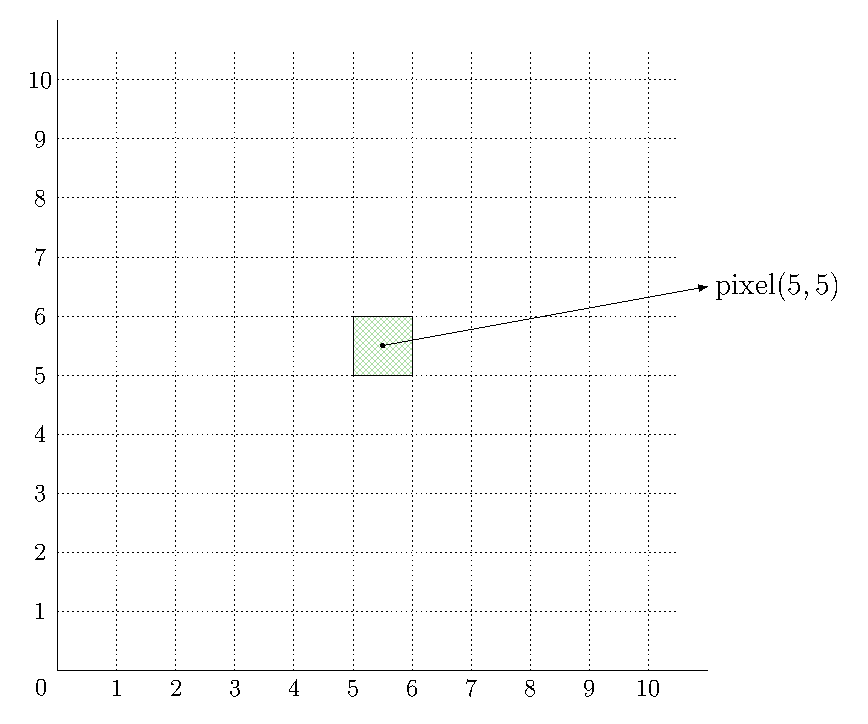
\includegraphics[scale=0.8]{History/pixel-grid.pdf}
\end{center}


%
 Ο φωτισμός διαδοχικών pixels σχηματίζει συγκεκριμένα σχήματα π.χ. ευθεία γραμμή.
Τα pixels έχουν πάντα ακέραιες συντεταγμένες. Εάν δοθεί εντολή να φωτιστεί το pixel $(10.33, 20.72)$ θα γίνει στρογγύλευση και το pixel που θα φωτιστεί τελικά θα είναι $(10, 21)$. Αυτή η διαδικασία της στρογγύλευσης προξενεί τις γραμμές να εμφανίζονται σκαλωτά και ονομάζονται ``jaggies". Το φαινόμενο αυτό είναι αισθητό σε συστήματα με χαμηλή ανάλυση.


\begin{center}
	
\includegraphics[scale=1.3]{History/jaggers.pdf}
\end{center}